
\section{Interazione con OBP}

L'interfaccia di OBP è una interfaccia RESTful\footnote{L'interfaccia di OBP, in realtà, è in sola lettura. Estendiamo il suo funzionamento anche alla scrittura (inserimento di informazioni nel back-end), poiché l'estensione delle sue funzionalità in questo senso è, almeno logicamente, immediata.}, in cui i dati vengono trasmessi in formato json, e l'autenticazione è gestita tramite protocollo OAuth\cite{oauthrfc} (versione 1.0, prima revisione).

Il protocollo OAuth si basa sul modello client/server, e permette al client di accedere ad una risorsa protetta situata sul server e di propriet\`a di una terza entit\`a senza che questa (detta ``proprietario della risorsa'') debba condividere le proprie credenziali di accesso al server con il client.

In OBP i ruoli sono ripartiti nel seguente modo:
\begin{description}
	\item[Client] un'applicazione di terze parti che desideri accedere in lettura o in scrittura ai conti correnti presso la filiale (come il sistema HBS);
	\item[Server] l'API di OBP (e il back-end della banca soggiacente);
	\item[Resource owner] un correntista presso la banca iscritto a HBS;
	\item[Protected resource] un conto corrente di un correntista presso la banca;
	\item[Credentials] le credenziali di accesso alla banca del correntista;
	\item[Token] identificativo univoco fornito dal server al client.
\end{description}

In HBS il token per l'accesso ad un account del back-end della banca viene creato alla registrazione dell'utente, e associato all'account HBS del cliente.
La procedura per l'ottenimento del token \`e illustrata in figura \ref{fig:oauth:token}.

\begin{figure*}[h]
    \centering
	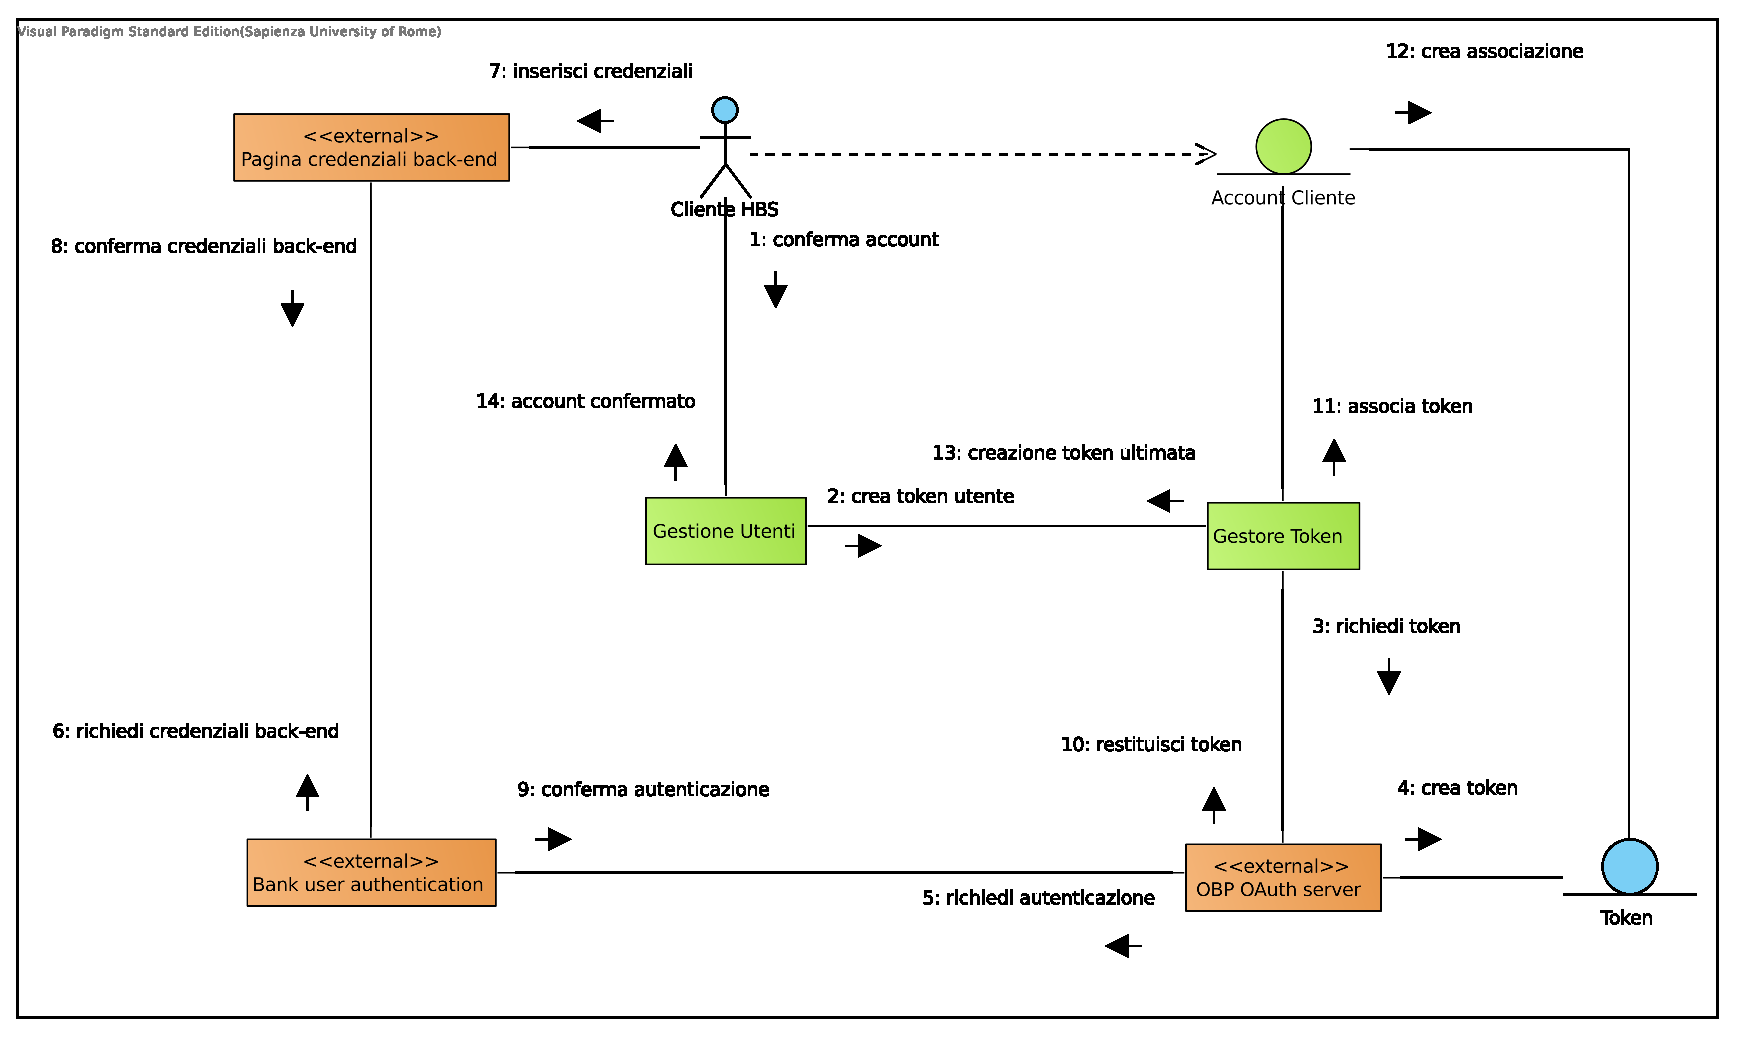
\includegraphics[width=\textwidth]{Images/Ottenimento_Token.eps}
    \caption{Diagramma di comunicazione illustrante la procedura per l'ottenimento del token.}
    \label{fig:oauth:token}
\end{figure*}

Inserire un'operazione bancaria nel back-end della banca avviene con il seguente messaggio:
\begin{lstlisting}[basicstyle=\ttfamily]
POST /accounts/[ACCOUNT_ID]/transactions HTTP/1.1
[header]

{
    "this_account": {
        "id": [id account],
        "number": [numero conto],
        "IBAN": [iban conto],
        "swift_bic": [codice swift],
        "bank": {
            "national_identifier": [identificatore banca],
            "name": [nome banca]
        }
    },
    "other_account": {
        "holder": {
            "name": [nome beneficiario]
        },
        "number": [numero conto beneficiario],
        "IBAN": [iban beneficiario],
        "swift_bic": [codice swift],
        "bank": {
            "national_identifier": [identificatore istituto beneficiario],
            "name": [nome istituto beneficiario]
        },
    },
    "details": {
        "posted_by_user_id": [id utente],
        "posted_by_ip_address": [ip terminale],
        "type": "cash",
        "description": [causale],
        "posted": [data esecuzione],
        "value": {
            "currency": [valuta],
            "amount": [cifra]
        }
    }
}
\end{lstlisting}
Il messaggio di risposta contiene informazioni riguardo l'avvenuta presa in carico dell'operazione da parte del back-end della banca.
